\chapter{Insiemi Frequenti e Regole d'Associazione}\label{ch:frequent-itemsets}
% Basato sulle slide del corso ("Mining insiemi frequenti -- Parte 1") e approfondimenti dal libro (Leskovec et al., cap. 6).

\section{Market-basket model e definizioni}\label{sec:mbm}
Nel \emph{market-basket model} ogni transazione (\emph{basket}) è un insieme di oggetti (\emph{item}). L'obiettivo è individuare \textbf{itemset frequenti}, cioè insiemi di item che compaiono assieme in molte transazioni, e derivarne \textbf{regole d'associazione} utili per descrivere co-occorrenze interessanti.

\paragraph{Supporto.} Sia $\mathcal{D}$ l'insieme dei basket (con $|\mathcal{D}|=N$) e sia $I=\{i_1,\dots,i_k\}$ un itemset. Il \textbf{supporto} assoluto di $I$ è
\[
\mathrm{supp}(I) = |\{ T\in\mathcal{D}\,:\, I\subseteq T\}|,\qquad \mathrm{supp}_\mathrm{rel}(I)=\frac{\mathrm{supp}(I)}{N}.
\]
Dato un valore soglia $\sigma$ (\emph{min-sup}), $I$ è detto \textbf{frequente} se $\mathrm{supp}(I)\ge \sigma$.

\paragraph{Soglia di supporto: trade-off.} Una soglia troppo alta può eliminare pattern interessanti; una troppo bassa produce un'esplosione di candidati difficili da analizzare e validare.

\section{Regole d'associazione}\label{sec:assoc}
Una \textbf{regola d'associazione} è un'implicazione $X\to j$, con $X$ itemset e $j$ un singolo item con $j\notin X$. Si estende naturalmente a $X\to Y$ con $X\cap Y=\varnothing$.

\subsection{Qualità di una regola}\label{subsec:qualita-regole}
\paragraph{Confidenza.} Con $\mathrm{supp}(\cdot)$ definito sopra, la confidenza di $X\to j$ è
\[
\mathrm{conf}(X\to j) = \frac{\mathrm{supp}(X\cup\{j\})}{\mathrm{supp}(X)} \;=\; P(j\mid X).\label{eq:confidence}
\]
\paragraph{Coverage.} $\mathrm{supp}(X)$ è detto anche \emph{coverage}: misura quanto spesso è applicabile la regola.
\paragraph{Interesse (o \emph{interest}).} Quantifica l'influenza di $X$ su $j$ come scostamento dalla prevalenza marginale di $j$:
\[
\mathrm{int}(X\to j) = \mathrm{conf}(X\to j) - \frac{\mathrm{supp}(\{j\})}{N}.
\]
\paragraph{Lift.} Confronta la co-occorrenza osservata con quella attesa in caso di indipendenza:
\[
\mathrm{lift}(X\to j) = \frac{N\cdot\mathrm{supp}(X\cup\{j\})}{\mathrm{supp}(X)\,\mathrm{supp}(\{j\})} \;=\; \frac{\mathrm{conf}(X\to j)}{\mathrm{supp}(\{j\})/N}.
\]
Valori $>1$ indicano associazione positiva, $<1$ negativa.

\paragraph{Nota.} Supporto e confidenza alti non implicano necessariamente interesse: regole ovvie (es. {pasta, pomodoro} $\to$ {pasta}) possono essere poco informative.

\subsection{Mini-esempio (dataset giocattolo)}\label{subsec:mini-esempio}
Sia $N=8$ e consideriamo item $\{b,c,j,m,p\}$. Supponiamo che $\mathrm{supp}(\{b\})=6$, $\mathrm{supp}(\{c\})=5$, $\mathrm{supp}(\{j\})=4$, $\mathrm{supp}(\{m\})=5$, $\mathrm{supp}(\{p\})=2$ e, tra le coppie, $\mathrm{supp}(\{b,c\})=4$, $\mathrm{supp}(\{c,j\})=3$, $\mathrm{supp}(\{c,m\})=2$, $\mathrm{supp}(\{m,p\})=2$, ecc. Per la regola $\{c,m\}\to b$ si ha
\[
\mathrm{conf}=\tfrac{\mathrm{supp}(\{b,c,m\})}{\mathrm{supp}(\{c,m\})}=\tfrac{2}{2}=1.0,\quad
\mathrm{lift}=\frac{8\cdot 2}{2\cdot 6}=1.33\,.
\]

\section{Insiemi frequenti chiusi e massimali}\label{sec:closed-maximal}
Sia $I$ frequente.
\begin{itemize}
  \item $I$ è \textbf{chiuso} se nessun suo super-insieme ha lo \emph{stesso} supporto di $I$.
  \item $I$ è \textbf{massimale} se nessun suo super-insieme è frequente.
\end{itemize}
Gli insiemi massimali sono (per definizione) chiusi; gli insiemi chiusi sono un sottoinsieme degli insiemi frequenti e consentono una rappresentazione più compatta senza perdere il supporto degli insiemi chiusi stessi.

\begin{figure}[htbp]
  \centering
  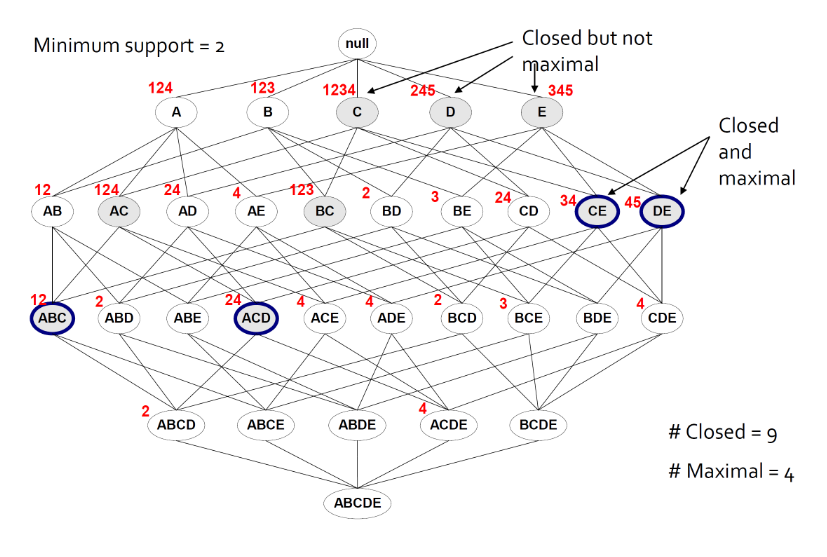
\includegraphics[width=0.8\textwidth]{images/insiemi_frequenti_massimale.png}
  \caption[Itemset lattice (minsup 2)]%
  {Grafo degli itemset con minsup $=2$. Un itemset è \emph{frequente} se il suo supporto è \texorpdfstring{$\ge 2$}{>= 2};
  è \emph{chiuso} se nessun superinsieme ha lo stesso supporto; è \emph{massimale} se nessun superinsieme è frequente.
  Nell'esempio: alcuni chiusi (es. CE) e chiusi–massimali (CE, DE); conteggi indicati: \#closed = 9, \#maximal = 4.}
  \label{fig:ifm}
\end{figure}


\section{Proprietà anti-monotona e Principio di Apriori}\label{sec:apriori-principle}
Per itemset $S\subseteq I$ vale l'\textbf{anti-monotonicità del supporto}:
\[
\mathrm{supp}(I)\le \mathrm{supp}(S).\label{eq:anti-mon}
\]
Da cui il \textbf{Principio di Apriori}: se un itemset $I$ è frequente, ogni suo sottoinsieme è frequente; equivalentemente, se $I$ non è frequente, nessun suo super-insieme può esserlo. Questa proprietà consente un \emph{pruning} efficace dello spazio dei candidati.

\section{Algoritmo Apriori}\label{sec:apriori}
Ricerca bottom-up per cardinalità crescente.
\begin{enumerate}
  \item Calcola l'insieme $L_1$ degli item singoli frequenti.
  \item Per $k=1,2,\dots$:
  \begin{enumerate}
    \item \textbf{Join}: genera $C_{k+1}$ (candidati di taglia $k{+}1$) con self-join di $L_k$.
    \item \textbf{Prune}: elimina da $C_{k+1}$ gli itemset che contengono sottoinsiemi di taglia $k$ non frequenti (per \S\ref{sec:apriori-principle}).
    \item \textbf{Conteggio}: calcola $\mathrm{supp}(\cdot)$ dei candidati scorrendo il DB e costruisci $L_{k+1}=\{c\in C_{k+1}: \mathrm{supp}(c)\ge\sigma\}$.
  \end{enumerate}
  \item Arresta quando $C_{k+1}=\varnothing$.
\end{enumerate}

\subsection{Apriori: esempio (minsup = 2)}\label{subsec:apriori-esempio}
Consideriamo $N=8$ basket e gli item $\{b,c,j,m,p\}$. I supporti degli item singoli sono:
\begin{center}
\begin{tabular}{@{}lccccc@{}}
\toprule
Item & $b$ & $c$ & $j$ & $m$ & $p$ \\
\midrule
$\mathrm{supp}(\cdot)$ & 6 & 5 & 4 & 5 & 2 \\
\bottomrule
\end{tabular}
\end{center}
Con minsup $=2$, tutti e cinque gli item sono frequenti, quindi $L_1=\{b,c,j,m,p\}$. \emph{(Dati come nelle slide)}.

\paragraph{Passo $k=1\to2$: generazione $C_2$ e pruning.}
$C_2$ si ottiene con self-join di $L_1$ e contiene tutte le coppie possibili:
\[
\{b,c\},\{b,j\},\{b,m\},\{b,p\},\{c,j\},\{c,m\},\{c,p\},\{j,m\},\{j,p\},\{m,p\}.
\]
Dai conteggi nel DB (come in tabella delle slide) si ottengono i supporti:
\begin{center}
\begin{tabular}{@{}lcccccccccc@{}}
\toprule
Itemset & $\{b,c\}$ & $\{b,j\}$ & $\{b,m\}$ & $\{b,p\}$ & $\{c,j\}$ & $\{c,m\}$ & $\{c,p\}$ & $\{j,m\}$ & $\{j,p\}$ & $\{m,p\}$ \\
\midrule
$\mathrm{supp}(\cdot)$ & 4 & 2 & 4 & 1 & 3 & 2 & 0 & 2 & 1 & 2 \\
\bottomrule
\end{tabular}
\end{center}
Applicando minsup, otteniamo $L_2=\{\{b,c\},\{b,j\},\{b,m\},\{c,j\},\{c,m\},\{j,m\},\{m,p\}\}$. 

\paragraph{Passo $k=2\to3$: generazione $C_3$ da $L_2$ (self-join) e pruning.}
Si combinano coppie con i primi $k-1$ item uguali (ordine lessicografico) e si rimuovono i candidati che hanno qualche sottoinsieme di taglia 2 non in $L_2$ (Principio di Apriori, \S\ref{sec:apriori-principle}). I candidati che restano sono:
\[
C_3=\{\{b,c,j\},\{b,c,m\},\{b,j,m\},\{c,j,m\}\}.
\]
Conteggiando i supporti sul DB (slide):
\begin{center}
\begin{tabular}{@{}lcccc@{}}
\toprule
Itemset & $\{b,c,j\}$ & $\{b,c,m\}$ & $\{b,j,m\}$ & $\{c,j,m\}$ \\
\midrule
$\mathrm{supp}(\cdot)$ & 2 & 2 & 1 & 1 \\
\bottomrule
\end{tabular}
\end{center}
Quindi $L_3=\{\{b,c,j\},\{b,c,m\}\}$.

\paragraph{Passo $k=3\to4$: generazione $C_4$ e arresto.}
L’unico candidato unibile è $\{b,c,j,m\}$, ma il suo supporto vale $1<2$, dunque non è frequente e $L_4=\varnothing$. L’algoritmo termina.

\paragraph{Riassunto dell’esempio.}
\[
L_1=\{b,c,j,m,p\},\quad
L_2=\{\{b,c\},\{b,j\},\{b,m\},\{c,j\},\{c,m\},\{j,m\},\{m,p\}\},
\]
\[
L_3=\{\{b,c,j\},\{b,c,m\}\},\quad
L_4=\varnothing.
\]
L’anti-monotonicità del supporto permette il \emph{pruning} efficace a ogni livello, riducendo drasticamente i candidati da contare. 


\subsection{Generazione dei candidati}\label{subsec:candidate-gen}
Se gli item sono ordinati, due insiemi $A=(a_1,\dots,a_{k-1},x)$ e $B=(a_1,\dots,a_{k-1},y)$ in $L_k$ con $x<y$ producono il candidato $(a_1,\dots,a_{k-1},x,y)$. Il passo di \emph{prune} scarta i candidati che hanno almeno un sottoinsieme di taglia $k$ non presente in $L_k$.

\paragraph{Esempio (schema).} Da $L_2=\{\{b,c\},\{b,j\},\{b,m\},\{c,j\},\{c,m\},\{j,m\},\{m,p\}\}$ si generano candidati di taglia 3 come $\{b,c,j\}$, $\{b,c,m\}$, $\{b,j,m\}$, $\{c,j,m\}$, ecc., poi si eliminano quelli che contengono coppie non frequenti.

\section{Ottimizzazioni di Apriori}\label{sec:apriori-opt}
\subsection{Hashing in bucket: PCY}\label{subsec:pcy}
Alla prima passata si contano i singoli item e, parallelamente, si proiettano tutte le coppie in bucket tramite una funzione hash. I bucket con supporto sotto soglia vengono marcati come non frequenti: alla seconda passata, una coppia $(i,j)$ è candidata solo se \emph{entrambi} gli item sono frequenti e il bucket hash di $(i,j)$ è frequente. Ciò riduce notevolmente $|C_2|$.

\subsection{Partizionamento del DB: SON}\label{subsec:son}
Divide il dataset in partizioni; su ciascuna partizione si esegue Apriori con min-sup scalato (proporzionale alla frazione di transazioni della partizione). L'unione degli insiemi frequenti locali fornisce i candidati globali, che vengono poi verificati su tutto il DB. L'algoritmo è adatto a calcolo distribuito.

\subsection{Campionamento e frontiera negativa: Toivonen}\label{subsec:toivonen}
Si esegue Apriori su un campione casuale $S$ con soglia più bassa ($\sigma'$); si ottiene un insieme di itemset frequenti in $S$ e la \emph{frontiera negativa}: insiemi non frequenti in $S$ i cui \emph{immediati} sottoinsiemi sono frequenti. Se nessun elemento della frontiera negativa risulta frequente sull'intero DB, i frequenti di $S$ sono la risposta; altrimenti si ripete con un nuovo campione (per evitare falsi negativi), regolando $\sigma'$.

\section{Perch\'e andare oltre Apriori}\label{sec:oltre-apriori}
Apriori richiede (i) generare esplicitamente i candidati $C_k$ a ogni livello e (ii) pi\`u passate sul database per calcolare i supporti. Con soglie basse o molti pattern, il numero di candidati esplode e le scansioni diventano costose. \textbf{FP-Growth} evita entrambi: rappresenta il DB in modo compatto (\emph{FP-tree}) e \emph{fa crescere} i pattern frequenti senza generare $C_k$.

\section{FP-Growth: idea di base}\label{sec:fpgrowth}
\begin{enumerate}
  \item \textbf{Costruzione FP-tree} (\emph{Frequent Pattern tree}): scansiona il DB per ottenere i supporti degli item, scarta quelli con supporto $<\sigma$, ordina gli item per supporto decrescente e inserisci le transazioni nell’albero condividendo i prefissi comuni. Mantieni una \emph{header table} con link ai nodi per item.
  \item \textbf{Pattern-growth}: per ogni item $x$ (dall’ultimo al primo nell’ordine per supporto) estrai la \emph{pattern base condizionale} di $x$ dai cammini che portano a $x$, costruisci l’\emph{FP-tree condizionale} e ripeti ricorsivamente. I pattern trovati si concatenano con $x$.
\end{enumerate}
Servono in genere \textbf{due passate} sul DB (una per i conteggi degli item, una per costruire l’albero); poi si lavora su strutture in memoria.

\subsection{Costruzione dell'FP-tree}\label{subsec:costruzione-fptree}
\begin{enumerate}
  \item \textbf{Prima passata}: calcola $\mathrm{supp}(i)$ per ogni item; elimina gli item con $\mathrm{supp}(i)<\sigma$.
  \item \textbf{Ordina} gli item per supporto decrescente (tie-break fisso) e \textbf{riordina} ogni transazione seguendo lo stesso ordine.
  \item \textbf{Inserisci} ciascuna transazione nell’albero a partire dalla radice: percorri/crea i nodi lungo il prefisso ordinato, incrementando i contatori dei nodi e aggiornando i \emph{node link} nella header table.
\end{enumerate}
\emph{Propriet\`a}: l’FP-tree conserva l’informazione necessaria a ricostruire i supporti dei pattern frequenti ed \`e molto compatto se molte transazioni condividono prefissi.

\subsection{Esempio di FP-Growth}\label{subsec:fpg-example}
Soglia $\sigma=3$. Dalla prima passata otteniamo gli item frequenti (con supporto) in ordine decrescente:
\[
f:4,\quad c:4,\quad a:3,\quad b:3,\quad m:3,\quad p:3.
\]
Ogni transazione viene \textbf{riordinata} secondo l’ordine $f\!\succ c\!\succ a\!\succ b\!\succ m\!\succ p$ ed \textbf{inserita} nell’FP-tree, aggregando i prefissi per incrementare i contatori.

\paragraph{Header table iniziale.}
\begin{center}
\begin{tabular}{@{}lcccccc@{}}
\toprule
Item & $f$ & $c$ & $a$ & $b$ & $m$ & $p$ \\
\midrule
$\mathrm{supp}(\cdot)$ & 4 & 4 & 3 & 3 & 3 & 3 \\
\bottomrule
\end{tabular}
\end{center}

\begin{figure}[htbp]
  \centering
  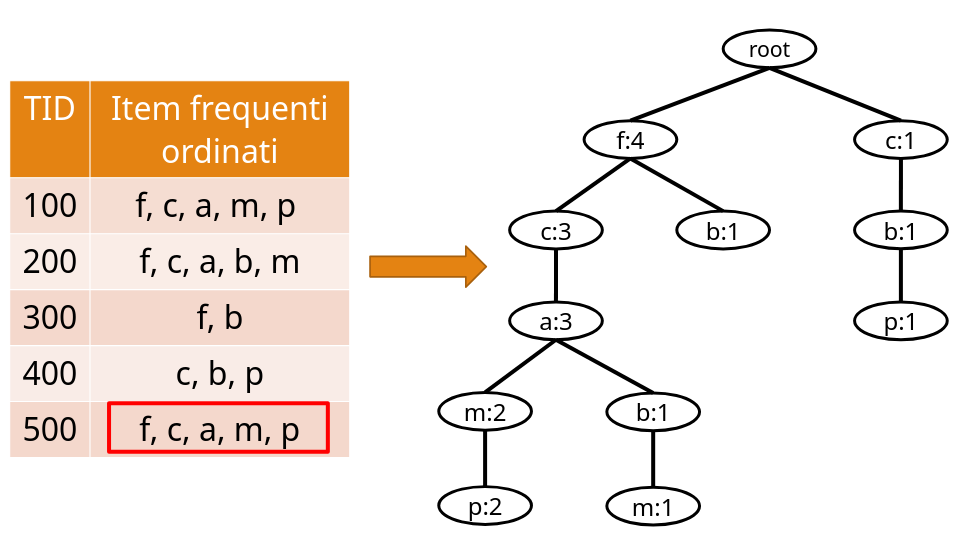
\includegraphics[width=0.92\textwidth]{images/fp-growth-complete.png}
  \caption{Costruzione dell’FP-tree: a sinistra le transazioni con gli item frequenti ordinati; a destra l’albero ottenuto condividendo i prefissi e incrementando i contatori dei nodi. L’ultima transazione (TID 500) segue il percorso f $\rightarrow$ c $\rightarrow$ a $\rightarrow$ m $\rightarrow$ p e aggiorna i relativi nodi.}
  \label{fig:fp-growth-complete}
\end{figure}

\paragraph{Visita per pattern-growth.}
Si processano gli item \emph{dal meno frequente al pi\`u frequente} nell’ordine della header table (a parit\`a, dall’ultimo al primo):
\[
p \rightarrow m \rightarrow b \rightarrow a \rightarrow c \rightarrow f.
\]

\paragraph{Come si espande un item $x$ (pattern-growth).}
\begin{enumerate}
  \item \textbf{Pattern base condizionale di $x$.} Segui i \emph{node link} di $x$ e,
        per ogni nodo $x$, prendi il cammino dalla radice al \emph{genitore} di $x$
        (escludi $x$). Assegna a quel cammino un \emph{peso} uguale al contatore del nodo $x$.
        % Multinsieme di cammini pesati: quali prefissi compaiono insieme a $x$ e quanto spesso.
  \item \textbf{FP-tree condizionale di $x$.} Dai cammini pesati:
        (i) somma i pesi per ogni item e \emph{rimuovi} quelli con supporto $<\sigma$;
        (ii) ordina gli item per supporto decrescente; 
        (iii) inserisci i cammini (con pesi) costruendo l’albero $T_x$.
  \item \textbf{Ricorsione e output.} I pattern frequenti che \emph{contengono} $x$
        sono $\{x\}$ unito a ciascun pattern frequente trovato in $T_x$.
        \emph{Caso speciale (cammino unico)}: se $T_x$ è una sola path,
        tutte le combinazioni dei suoi nodi sono frequenti; il supporto è il \emph{minimo} dei contatori lungo la combinazione.
\end{enumerate}

\begin{figure}[htbp]
  \centering
  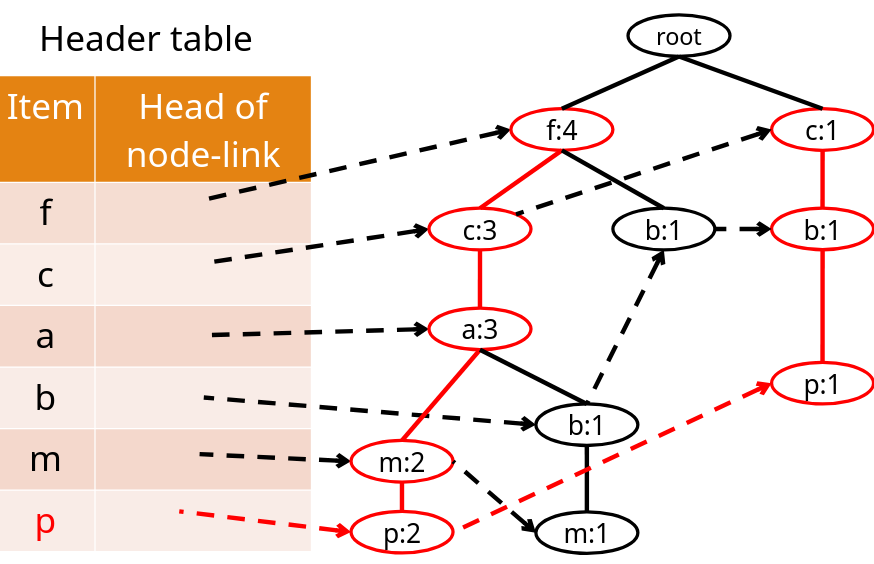
\includegraphics[width=0.9\textwidth]{images/fp-growth-links.png}
  \caption{Header table e node-link per l’item $p$: i puntini tratteggiati collegano le occorrenze di $p$ nell’FP-tree. Seguendo i node-link si raccolgono i cammini verso la radice (senza $p$) con i rispettivi contatori: questa è la pattern base condizionale di $p$, da cui si costruisce l’FP-tree condizionale $T_p$.}
  \label{fig:fp-growth-links}
\end{figure}

\paragraph{Esempio 1: item $p$.}
Supponiamo che, seguendo i \emph{node link} di $p$, si incontrino i cammini verso radice:
\[
\langle f,c,a,m\rangle:2 \quad \text{e} \quad \langle c,b\rangle:1.
\]
La \textbf{base condizionale} di $p$ \`e quindi $\{\langle f,c,a,m\rangle \text{ con peso } 2,\ \langle c,b\rangle \text{ con peso } 1\}$. Con $\sigma=3$ nessun sotto-pattern che include $p$ raggiunge la soglia (pesi massimi 2 e 1), dunque \emph{nessun} pattern frequente contiene $p$.

\paragraph{Esempio 2: item $m$.}
Cammini verso $m$ (esempio coerente con le slide):
\[
\langle f,c,a\rangle:2,\quad \langle f,c\rangle:1.
\]
La base condizionale di $m$ \`e $\{\langle f,c,a\rangle:2,\ \langle f,c\rangle:1\}$. Frequenze condizionali:
\[
\mathrm{supp}_{\mathrm{cond}}(f)=3,\ \mathrm{supp}_{\mathrm{cond}}(c)=3,\ \mathrm{supp}_{\mathrm{cond}}(a)=2.
\]
Con $\sigma=3$ risultano frequenti i pattern $\{m,f\}$, $\{m,c\}$ e, proseguendo, $\{m,f,c\}$ con supporto $3$ (intersezione dei cammini). 

\paragraph{Esempio 3: item $b$.}
Cammini verso $b$:
\[
\langle f,c,a\rangle:2,\quad \langle c\rangle:1.
\]
Base condizionale di $b$: $\{\langle f,c,a\rangle:2,\ \langle c\rangle:1\}$. Frequenze condizionali:
\[
\mathrm{supp}_{\mathrm{cond}}(c)=3,\ \mathrm{supp}_{\mathrm{cond}}(f)=2,\ \mathrm{supp}_{\mathrm{cond}}(a)=2.
\]
Con $\sigma=3$ si ottiene $\{b,c\}$ frequente; combinazioni con $f$ o $a$ non superano la soglia.

\section{Confronto: FP-Growth vs Apriori}\label{subsec:confronto-fp-apriori}
\begin{table}[htbp]
\centering
\begin{tabular}{@{}p{0.28\textwidth}p{0.33\textwidth}p{0.33\textwidth}@{}}
\toprule
\textbf{Aspetto} & \textbf{Apriori} & \textbf{FP-Growth} \\
\midrule
Generazione candidati &
Sì: crea $C_k$ a ogni livello (rischio di esplosione combinatoria) &
No: crescita diretta dei pattern dall’FP-tree \\
Accessi al DB &
Molte passate (una per ogni $k$) &
Tipicamente 2 passate, poi si lavora in memoria \\
Strutture dati principali &
Liste di candidati e conteggi &
FP-tree + header table (node-link) \\
Quando preferirlo &
DB piccoli/sparsi, soglie alte, ambienti distribuiti molto semplici &
DB densi, soglie basse, molti prefissi condivisi (compressione efficace) \\
Note pratiche &
Pruning con principio di Apriori, implementazione semplice &
Evita i candidati; molto veloce se l’FP-tree è compatto \\
\bottomrule
\end{tabular}
\caption{Confronto sintetico tra Apriori e FP-Growth.}
\label{tab:apriori-vs-fpgrowth}
\end{table}